\documentclass[12pt]{article}					% Začátek dokumentu
\usepackage{../../MFFStyle}					    % Import stylu
\usetikzlibrary{arrows}

\begin{document}
\definecolor{eqeqeq}{rgb}{0.8784313725490196,0.8784313725490196,0.8784313725490196}
\begin{priklad}[1]
    Rozhodněte, zda je následující graf rovinný:

    \hfill\hfill
    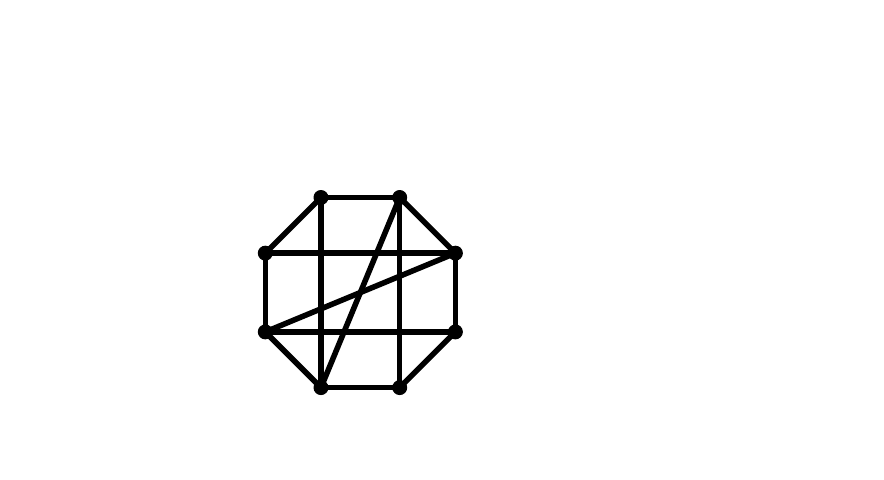
\begin{tikzpicture}[line cap=round,line join=round,>=triangle 45,x=1.0cm,y=1.0cm]
        \clip(-3.72486683943315,-0.81340955624387) rectangle (6.790963617078251,4.570801992285996);
        \draw [line width=2.pt] (-0.7071067811865475,1.7071067811865477)-- (0.,2.414213562373095);
        \draw [line width=2.pt] (0.,2.414213562373095)-- (1.,2.414213562373095);
        \draw [line width=2.pt] (1.,2.414213562373095)-- (1.7071067811865475,1.7071067811865472);
        \draw [line width=2.pt] (1.7071067811865475,1.7071067811865472)-- (1.7071067811865475,0.7071067811865475);
        \draw [line width=2.pt] (1.7071067811865475,0.7071067811865475)-- (1.,0.);
        \draw [line width=2.pt] (1.,0.)-- (0.,0.);
        \draw [line width=2.pt] (0.,0.)-- (-0.7071067811865477,0.7071067811865478);
        \draw [line width=2.pt] (-0.7071067811865477,0.7071067811865478)-- (-0.7071067811865475,1.7071067811865477);
        \draw [line width=2.pt] (-0.7071067811865475,1.7071067811865477)-- (1.7071067811865475,1.7071067811865472);
        \draw [line width=2.pt] (1.7071067811865475,1.7071067811865472)-- (-0.7071067811865477,0.7071067811865478);
        \draw [line width=2.pt] (-0.7071067811865477,0.7071067811865478)-- (1.7071067811865475,0.7071067811865475);
        \draw [line width=2.pt] (0.,2.414213562373095)-- (0.,0.);
        \draw [line width=2.pt] (0.,0.)-- (1.,2.414213562373095);
        \draw [line width=2.pt] (1.,2.414213562373095)-- (1.,0.);
        \begin{scriptsize}
                \draw [fill=black] (0.,0.) circle (2.5pt);
                \draw [fill=black] (1.,0.) circle (2.5pt);
                \draw [fill=black] (1.7071067811865475,0.7071067811865475) circle (2.5pt);
                \draw [fill=black] (1.7071067811865475,1.7071067811865472) circle (2.5pt);
                \draw [fill=black] (1.,2.414213562373095) circle (2.5pt);
                \draw [fill=black] (0.,2.414213562373095) circle (2.5pt);
                \draw [fill=black] (-0.7071067811865475,1.7071067811865477) circle (2.5pt);
                \draw [fill=black] (-0.7071067811865477,0.7071067811865478) circle (2.5pt);
        \end{scriptsize}
    \end{tikzpicture}
    \hfill\ 

    \begin{reseni}
        Graf překreslíme rovinně (tj. je rovinný):

        \hfill\hfill\hfill
        \begin{tikzpicture}[line cap=round,line join=round,>=triangle 45,x=1.0cm,y=1.0cm]
                \clip(-3.72486683943315,-0.81340955624387) rectangle (6.790963617078251,4.570801992285996);
                \draw [line width=2.pt,color=eqeqeq] (0.,2.414213562373095)-- (0.,0.);
                \draw [line width=2.pt,color=eqeqeq] (0.,0.)-- (1.,2.414213562373095);
                \draw [line width=2.pt,color=eqeqeq] (1.,2.414213562373095)-- (1.,0.);
                \draw [line width=2.pt] (-0.7071067811865475,1.7071067811865477)-- (0.,2.414213562373095);
                \draw [line width=2.pt] (0.,2.414213562373095)-- (1.,2.414213562373095);
                \draw [line width=2.pt] (1.,2.414213562373095)-- (1.7071067811865475,1.7071067811865472);
                \draw [line width=2.pt] (1.7071067811865475,1.7071067811865472)-- (1.7071067811865475,0.7071067811865475);
                \draw [line width=2.pt] (1.7071067811865475,0.7071067811865475)-- (1.,0.);
                \draw [line width=2.pt] (1.,0.)-- (0.,0.);
                \draw [line width=2.pt] (0.,0.)-- (-0.7071067811865477,0.7071067811865478);
                \draw [line width=2.pt] (-0.7071067811865477,0.7071067811865478)-- (-0.7071067811865475,1.7071067811865477);
                \draw [line width=2.pt] (-0.7071067811865475,1.7071067811865477)-- (1.7071067811865475,1.7071067811865472);
                \draw [line width=2.pt] (1.7071067811865475,1.7071067811865472)-- (-0.7071067811865477,0.7071067811865478);
                \draw [line width=2.pt] (-0.7071067811865477,0.7071067811865478)-- (1.7071067811865475,0.7071067811865475);
                \draw [shift={(-0.10231881686184105,1.2071067811865475)},line width=3.6pt]  plot[domain=1.4862347785451642:4.796950528634422,variable=\t]({1.*1.211435479697765*cos(\t r)+0.*1.211435479697765*sin(\t r)},{0.*1.211435479697765*cos(\t r)+1.*1.211435479697765*sin(\t r)});
                \draw [shift={(-0.21872664166916597,1.5048131038047838)},line width=3.6pt]  plot[domain=0.641057627272188:4.85672951650995,variable=\t]({1.*1.5206261280007185*cos(\t r)+0.*1.5206261280007185*sin(\t r)},{0.*1.5206261280007185*cos(\t r)+1.*1.5206261280007185*sin(\t r)});
                \draw [shift={(1.7928174486437507,1.2071067811865475)},line width=3.6pt]  plot[domain=-2.1519310675455365:2.151931067545537,variable=\t]({1.*1.4441836060766422*cos(\t r)+0.*1.4441836060766422*sin(\t r)},{0.*1.4441836060766422*cos(\t r)+1.*1.4441836060766422*sin(\t r)});
                \begin{scriptsize}
                        \draw [fill=black] (0.,0.) circle (2.5pt);
                        \draw [fill=black] (1.,0.) circle (2.5pt);
                        \draw [fill=black] (1.7071067811865475,0.7071067811865475) circle (2.5pt);
                        \draw [fill=black] (1.7071067811865475,1.7071067811865472) circle (2.5pt);
                        \draw [fill=black] (1.,2.414213562373095) circle (2.5pt);
                        \draw [fill=black] (0.,2.414213562373095) circle (2.5pt);
                        \draw [fill=black] (-0.7071067811865475,1.7071067811865477) circle (2.5pt);
                        \draw [fill=black] (-0.7071067811865477,0.7071067811865478) circle (2.5pt);
                \end{scriptsize}
        \end{tikzpicture}
        \hfill\hfill\hfill\ 
    \end{reseni}
\end{priklad}

\pagebreak

\begin{priklad}[2]
    Dokažte že Petersonův graf není rovinný 2 způsoby: Pomocí nerovinnosti $K_5$ a faktu, že kontrakce hrany zachovává rovinnost (pouze jedním směrem; kontrakcí můžeme z nerovinného grafu udělat rovinný ale ne opačně), a přímým aplikováním Kuratowského věty.

    \begin{reseni}[Kontrakce]
        Zkontrahujeme zvýrazněné hrany a dostaneme jistě $K_5$, tedy graf jistě nemohl být rovinný, protože by po zkontrahování byl stále rovinný, ale my jsme získaly nerovinný graf ($K_5$ je nerovinný ze zadání).

        \definecolor{aqaqaq}{rgb}{0.6274509803921569,0.6274509803921569,0.6274509803921569}
        \hfill
        \begin{tikzpicture}[line cap=round,line join=round,>=triangle 45,x=1.0cm,y=1.0cm, scale=2]
                \clip(-1.395902340376328,-0.42034084359615964) rectangle (2.8725235172344052,1.7651363654207133);
                \draw [line width=2.8pt] (0.,0.)-- (0.26016351515335095,0.3580843586233004);
                \draw [line width=2.8pt] (0.11193641577582276,0.8142804621407592)-- (-0.30901699437494734,0.9510565162951536);
                \draw [line width=2.8pt] (0.5,1.0962251596498143)-- (0.5,1.5388417685876266);
                \draw [line width=2.8pt] (0.8880635842241774,0.8142804621407591)-- (1.3090169943749475,0.9510565162951532);
                \draw [line width=2.8pt] (0.739836484846649,0.3580843586233004)-- (1.,0.);
                \draw [line width=1.2pt,color=aqaqaq] (0.739836484846649,0.3580843586233004)-- (0.11193641577582276,0.8142804621407592);
                \draw [line width=1.2pt,color=aqaqaq] (0.11193641577582276,0.8142804621407592)-- (0.8880635842241774,0.8142804621407591);
                \draw [line width=1.2pt,color=aqaqaq] (0.8880635842241774,0.8142804621407591)-- (0.26016351515335095,0.3580843586233004);
                \draw [line width=1.2pt,color=aqaqaq] (0.26016351515335095,0.3580843586233004)-- (0.5,1.0962251596498143);
                \draw [line width=1.2pt,color=aqaqaq] (0.5,1.0962251596498143)-- (0.739836484846649,0.3580843586233004);
                \draw [line width=1.2pt,color=aqaqaq] (-0.30901699437494734,0.9510565162951536)-- (0.5,1.5388417685876266);
                \draw [line width=1.2pt,color=aqaqaq] (0.5,1.5388417685876266)-- (1.3090169943749475,0.9510565162951532);
                \draw [line width=1.2pt,color=aqaqaq] (1.3090169943749475,0.9510565162951532)-- (1.,0.);
                \draw [line width=1.2pt,color=aqaqaq] (1.,0.)-- (0.,0.);
                \draw [line width=1.2pt,color=aqaqaq] (0.,0.)-- (-0.30901699437494734,0.9510565162951536);
                \begin{scriptsize}
                        \draw [fill=black] (0.,0.) circle (1.5pt);
                        \draw [fill=black] (1.,0.) circle (1.5pt);
                        \draw [fill=black] (1.3090169943749475,0.9510565162951532) circle (1.5pt);
                        \draw [fill=black] (0.5,1.5388417685876266) circle (1.5pt);
                        \draw [fill=black] (-0.30901699437494734,0.9510565162951536) circle (1.5pt);
                        \draw [fill=black] (0.26016351515335095,0.3580843586233004) circle (1.5pt);
                        \draw [fill=black] (0.5,1.0962251596498143) circle (1.5pt);
                        \draw [fill=black] (0.8880635842241774,0.8142804621407591) circle (1.5pt);
                        \draw [fill=black] (0.739836484846649,0.3580843586233004) circle (1.5pt);
                        \draw [fill=black] (0.11193641577582276,0.8142804621407592) circle (1.5pt);
                \end{scriptsize}
        \end{tikzpicture}
        \hfill\hfill\ 
    \end{reseni}

    \begin{reseni}[Kuratowského věta]
        Pokud si vezmu následující barevný podgraf (bez šedých hran), tak ten je zřejmě dělením $K_{3, 3}$, jelikož každý zelený bod je spojen s každým červeným po disjunktních (mimo krajní vrcholy) cestách (každému zelenému bodu jsem dal jinou barvu cest k červeným).


        \definecolor{qqffff}{rgb}{0.,1.,1.}
        \definecolor{qqwwzz}{rgb}{0.,0.4,0.6}
        \definecolor{qqqqcc}{rgb}{0.,0.,0.8}
        \definecolor{ffqqqq}{rgb}{1.,0.,0.}
        \definecolor{qqffqq}{rgb}{0.,1.,0.}
        \definecolor{aqaqaq}{rgb}{0.6274509803921569,0.6274509803921569,0.6274509803921569}
        \hfill\hfill\hfill
        \begin{tikzpicture}[line cap=round,line join=round,>=triangle 45,x=1.0cm,y=1.0cm, scale=2]
                \clip(-1.0093352450321649,-0.09527222408526043) rectangle (2.4784679238614724,1.6905182732623076);
                \draw [line width=1.2pt,color=qqqqcc] (0.,0.)-- (0.26016351515335095,0.3580843586233004);
                \draw [line width=1.2pt,color=qqqqcc] (0.11193641577582276,0.8142804621407592)-- (-0.30901699437494734,0.9510565162951536);
                \draw [line width=1.2pt,color=qqwwzz] (0.5,1.0962251596498143)-- (0.5,1.5388417685876266);
                \draw [line width=1.2pt,color=qqffff] (0.8880635842241774,0.8142804621407591)-- (1.3090169943749475,0.9510565162951532);
                \draw [line width=1.2pt,color=aqaqaq] (0.739836484846649,0.3580843586233004)-- (1.,0.);
                \draw [line width=1.2pt,color=qqwwzz] (0.739836484846649,0.3580843586233004)-- (0.11193641577582276,0.8142804621407592);
                \draw [line width=1.2pt,color=qqffff] (0.11193641577582276,0.8142804621407592)-- (0.8880635842241774,0.8142804621407591);
                \draw [line width=1.2pt,color=qqffff] (0.8880635842241774,0.8142804621407591)-- (0.26016351515335095,0.3580843586233004);
                \draw [line width=1.2pt,color=qqwwzz] (0.26016351515335095,0.3580843586233004)-- (0.5,1.0962251596498143);
                \draw [line width=1.2pt,color=qqwwzz] (0.5,1.0962251596498143)-- (0.739836484846649,0.3580843586233004);
                \draw [line width=1.2pt,color=aqaqaq] (-0.30901699437494734,0.9510565162951536)-- (0.5,1.5388417685876266);
                \draw [line width=1.2pt,color=qqwwzz] (0.5,1.5388417685876266)-- (1.3090169943749475,0.9510565162951532);
                \draw [line width=1.2pt,color=qqqqcc] (1.3090169943749475,0.9510565162951532)-- (1.,0.);
                \draw [line width=1.2pt,color=qqqqcc] (1.,0.)-- (0.,0.);
                \draw [line width=1.2pt,color=qqqqcc] (0.,0.)-- (-0.30901699437494734,0.9510565162951536);
                \begin{scriptsize}
                        \draw [fill=qqffqq] (0.,0.) circle (1.5pt);
                        \draw [fill=black] (1.,0.) circle (1.5pt);
                        \draw [fill=ffqqqq] (1.3090169943749475,0.9510565162951532) circle (1.5pt);
                        \draw [fill=black] (0.5,1.5388417685876266) circle (1.5pt);
                        \draw [fill=black] (-0.30901699437494734,0.9510565162951536) circle (1.5pt);
                        \draw [fill=ffqqqq] (0.26016351515335095,0.3580843586233004) circle (1.5pt);
                        \draw [fill=qqffqq] (0.5,1.0962251596498143) circle (1.5pt);
                        \draw [fill=qqffqq] (0.8880635842241774,0.8142804621407591) circle (1.5pt);
                        \draw [fill=black] (0.739836484846649,0.3580843586233004) circle (1.5pt);
                        \draw [fill=ffqqqq] (0.11193641577582276,0.8142804621407592) circle (1.5pt);
                \end{scriptsize}
        \end{tikzpicture}
        \hfill\hfill\hfill\hfill\ 
    \end{reseni}
\end{priklad}

\end{document}
